%%%%%%%%%%%%%%%%%%%%%%%%%%%%%%%%%%%%%%%%%%%%%%%%%%%%%%%%%%%%%%%%%%%%%%%%%%%%%%%%
\chapter{Proof of Concepts and Validation}\label{ch:validation}
%%%%%%%%%%%%%%%%%%%%%%%%%%%%%%%%%%%%%%%%%%%%%%%%%%%%%%%%%%%%%%%%%%%%%%%%%%%%%%%%

\section{Emulated Testbeds}



As proof of concepts for our tool, we are going to use Mininet's emulated testbeds. We automate these tests using scripts, so they are reproducible.  They are responsible for building the topology, run the SIMITAR traffic generator, collect \textit{pcaps} and perform the proposed proof of concept analysis.  We make four plots for each trace, where we compare the original and the synthetic trace. The first two we used just for visual comparison:  flows per second and bandwidth. To compare the quality of the realism of the generated traffic, we plot the Flows cumulative distribution function\cite{harpoon-paper}, and the Wavelet multiresolution analysis\cite{swing-paper}.  Tests on physical testbeds and network functions stay for future work.

\begin{table}[ht!]
	\centering
	\caption{Experiments specification table}
	\label{tab:specifications}
	\begin{tabular}{ll}
		\hline
		Processor            & Intel(R) Core(TM) i7-4770, 8 cores, CPU @ 3.40GHz \\
		RAM                  & 15.5 GB                                           \\
		HD                   & 1000 GB                                            \\
		Linux         & 4.8.0-59-generic                                  \\
		Ubuntu        & Ubuntu 16.10 (yakkety)                            \\
		SIMITAR       & v0.4.2 (Eulemur rubriventer)                      \\
		Mininet       & 2.3.0d1                                           \\
		Iperf         & iperf version 2.0.9 (1 June 2016) pthreads        \\
		Libtins       & 3.4-2                                             \\
		OpenDayLight v & 0.4.0-Beryllium                                   \\
		Octave        & 4.0.3                                             \\
		Pyshark              & 0.3.6.2                                           \\
		Wireshark            & 2.2.6+g32dac6a-2ubuntu0.16.10                     \\ \hline
	\end{tabular}
\end{table}


We use two different testbeds: a tree topology (figure~\ref{fig:topo-tree}), similar to tests performed by Swing\cite{swing-paper}\cite{background-traffic-matter}\cite{legotg-paper}, and a single hop connection of two hosts. Both topologies are SDN networks and have OpenDayLight Beryllium as the controller.  We present the complete specification of these experiments at the table ~\ref{tab:specifications}.
	
We generate the traffic on the host \textit{h1} with IPv4 address 10.0.0.1. The traffic is captured from the host interface with TCPdump in a \textit{pcap} format.  We organized the project directory tree as follows\footnote{ \href{https://github.com/AndersonPaschoalon/ProjetoMestrado/tree/master/Tests}{https://github.com/AndersonPaschoalon/ProjetoMestrado/tree/master/Tests} }: we placed the software at \texttt{SIMITAR}. We paced the validation tests, with short tutorials at \texttt{Tests} directory. The software documentation is at \texttt{Docs} directory. We organized the tests as python packages, configurable by a \texttt{config.py} file.


\begin{figure}[!ht]
	\centering
	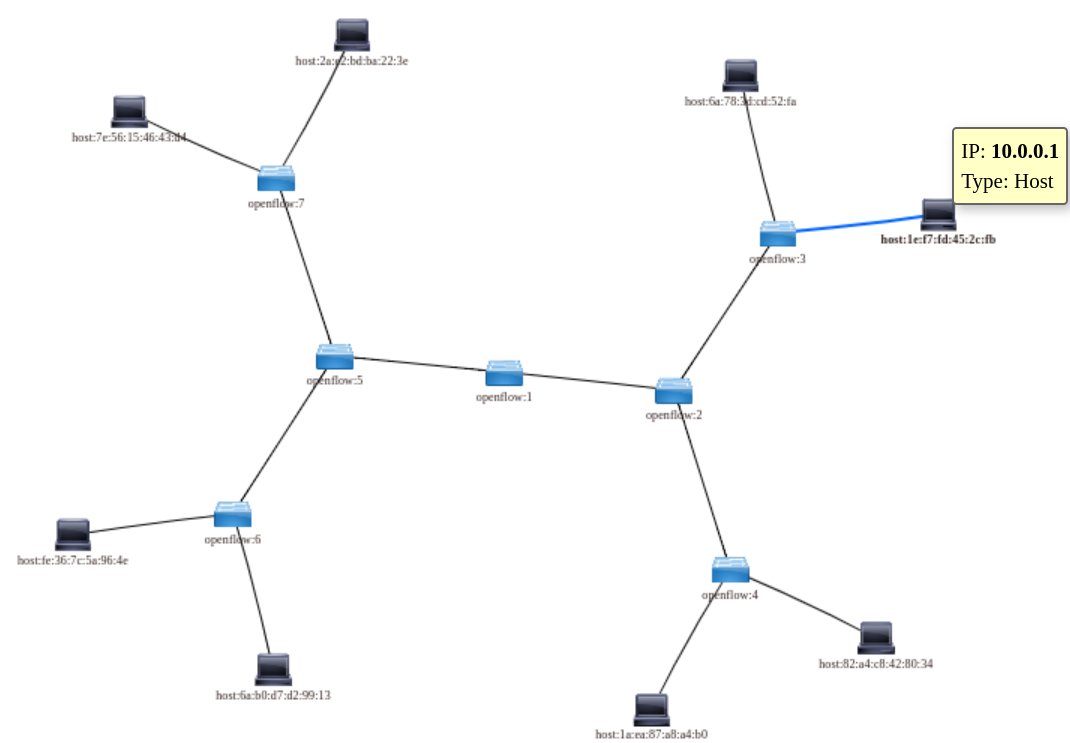
\includegraphics[scale=0.4]{figures/ch5/topo-tree}
	\caption{Tree SDN topology emulated by mininet, and controlled by OpenDayLight Beryllium}
	\label{fig:topo-tree}
\end{figure}

\begin{figure}[!ht]
	\centering
	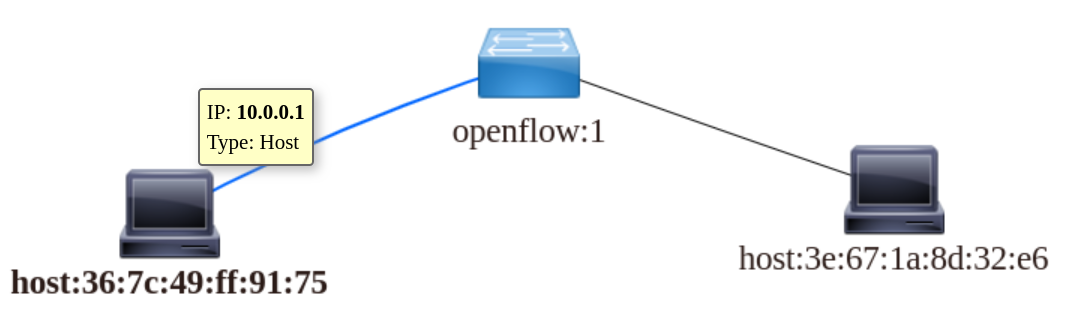
\includegraphics[scale=0.4]{figures/ch5/topo-simple}
	\caption{Single hop SDN topology emulated by mininet, and controlled by OpenDayLight Beryllium}
	\label{fig:topo-simple}
\end{figure}


\section{Simitar using Iperf and with skype-pcap}



\subsection{Single hop SDN topology}


\begin{figure}[t!]
	\centering
	\subfloat[\textit{skype-pcap}]{
		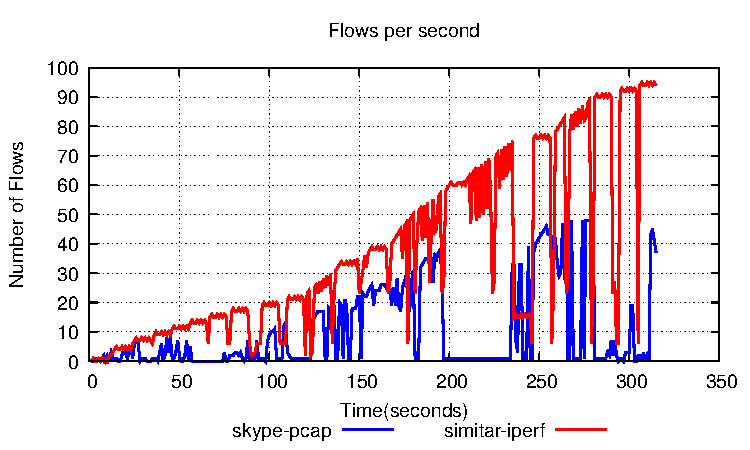
\includegraphics[width=77mm]{figures/ch5/iperfFlowsPs.pdf}
		\label{fig:iperf-single-flowps}
	}
	\hspace{0mm}
	\subfloat[\textit{bigFlows-pcap}]{
		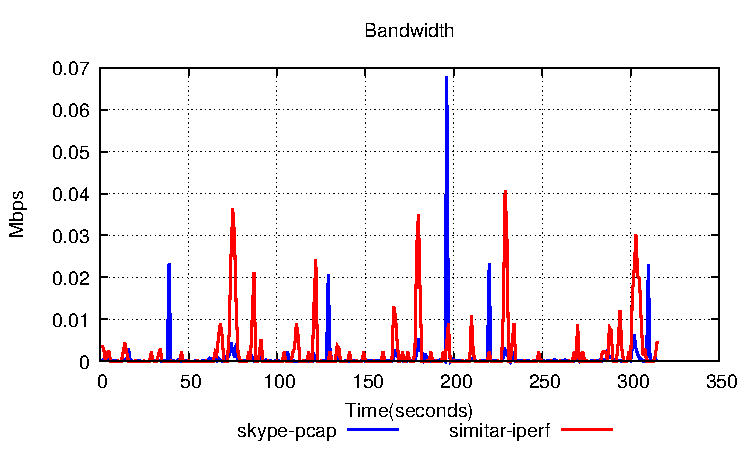
\includegraphics[width=77mm]{figures/ch5/iperfBandwidth.pdf}
		\label{fig:iperf-single-bw}
	}
	\hspace{0mm}
	\subfloat[\textit{lan-diurnal-pcap}]{
		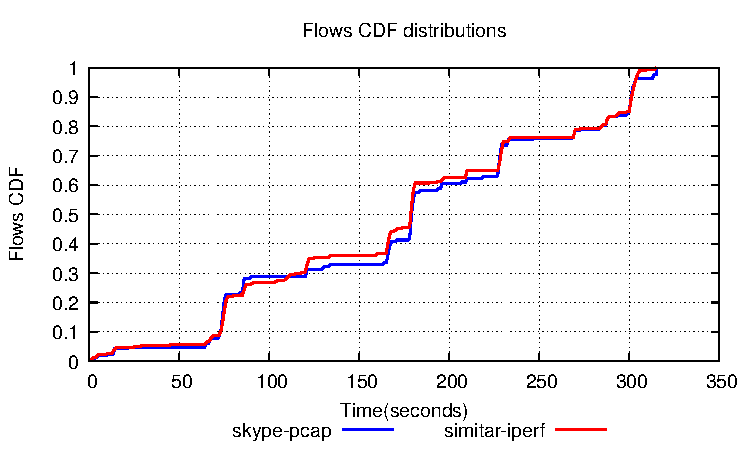
\includegraphics[width=77mm]{figures/ch5/iperfFlowCdf.pdf}
		\label{fig:iperf-single-flowcdf}
	}
	\hspace{0mm}
	\subfloat[\textit{wan-pcap}]{
		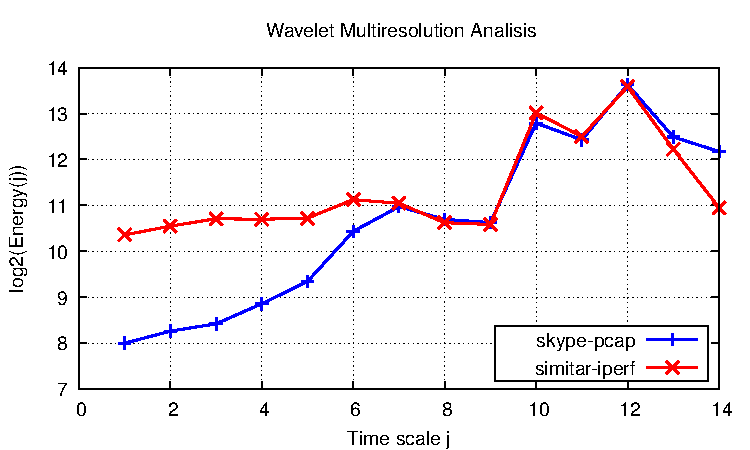
\includegraphics[width=77mm]{figures/ch5/iperfWaveletMREA.pdf}
		\label{fig:iperf-single-wavelet}
	}
	\caption{caption}
	\label{fig:iperf-single}
\end{figure}



\subsection{Tree SDN topology}


\begin{figure}[t!]
	\centering
	\subfloat[\textit{skype-pcap}]{
		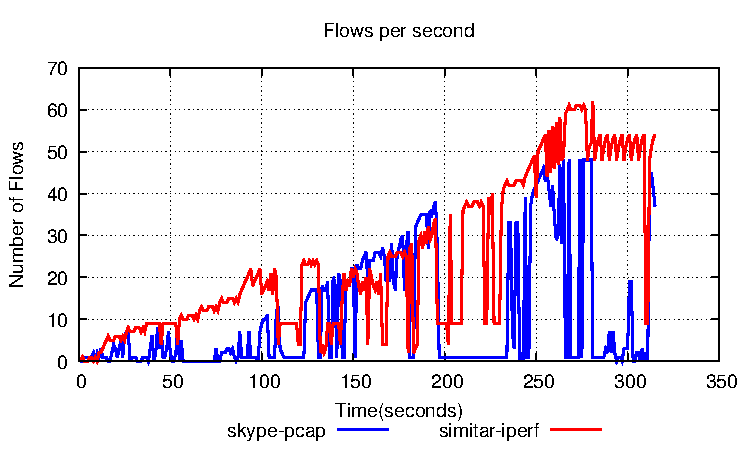
\includegraphics[width=77mm]{figures/ch5/iperftreeFlowsPs.pdf}
		\label{fig:iperf-flowps}
	}
	\hspace{0mm}
	\subfloat[\textit{bigFlows-pcap}]{
		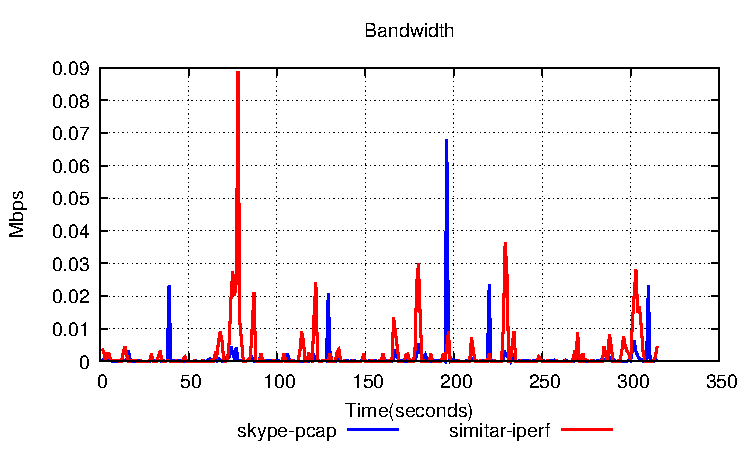
\includegraphics[width=77mm]{figures/ch5/iperftreeBandwidth.pdf}
		\label{fig:iperf-bw}
	}
	\hspace{0mm}
	\subfloat[\textit{lan-diurnal-pcap}]{
		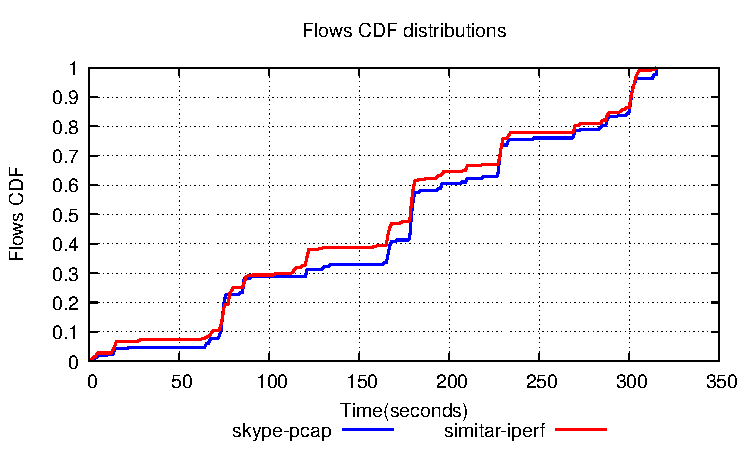
\includegraphics[width=77mm]{figures/ch5/iperftreeFlowCdf.pdf}
		\label{fig:iperf-flowcdf}
	}
	\hspace{0mm}
	\subfloat[\textit{wan-pcap}]{
		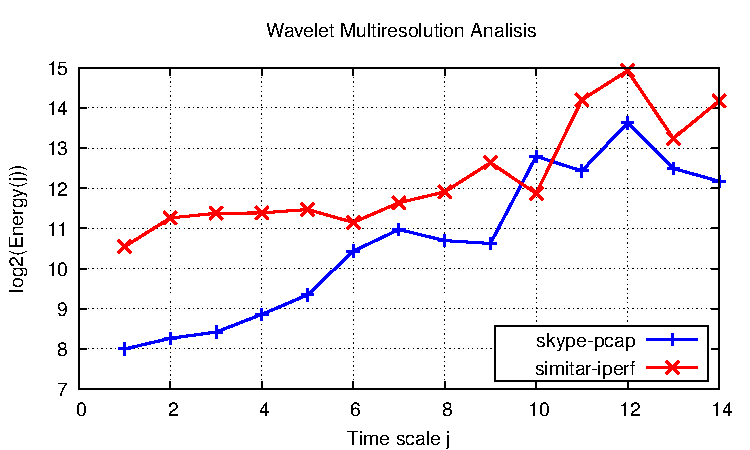
\includegraphics[width=77mm]{figures/ch5/iperftreeWaveletMREA.pdf}
		\label{fig:iperf-tree-wavelet}
	}
	\caption{caption}
	\label{fig:iperf-tree}
\end{figure}



\section{Simitar using Libtins with skype-pcap}


\begin{figure}[t!]
	\centering
	\subfloat[\textit{skype-pcap}]{
		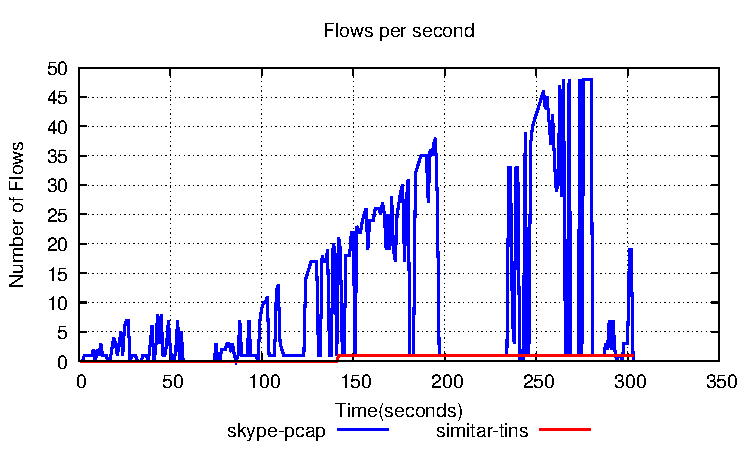
\includegraphics[width=77mm]{figures/ch5/tinsFlowsPs.pdf}
		\label{fig:tins-single-flowps}
	}
	\hspace{0mm}
	\subfloat[\textit{bigFlows-pcap}]{
		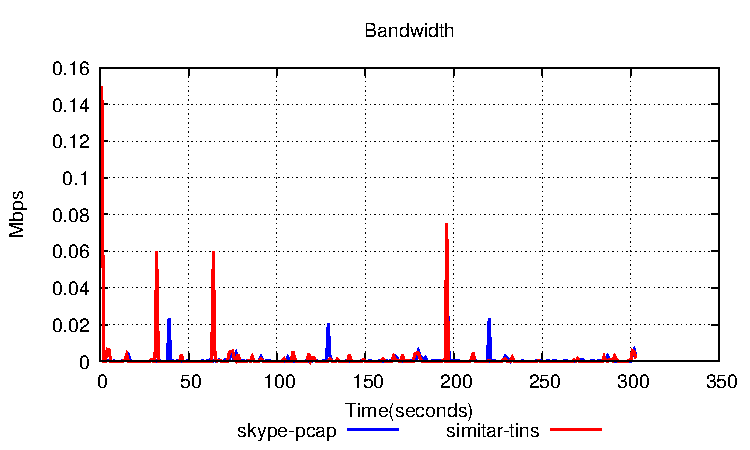
\includegraphics[width=77mm]{figures/ch5/tinsBandwidth.pdf}
		\label{fig:tins-single-bw}
	}
	\hspace{0mm}
	\subfloat[\textit{lan-diurnal-pcap}]{
		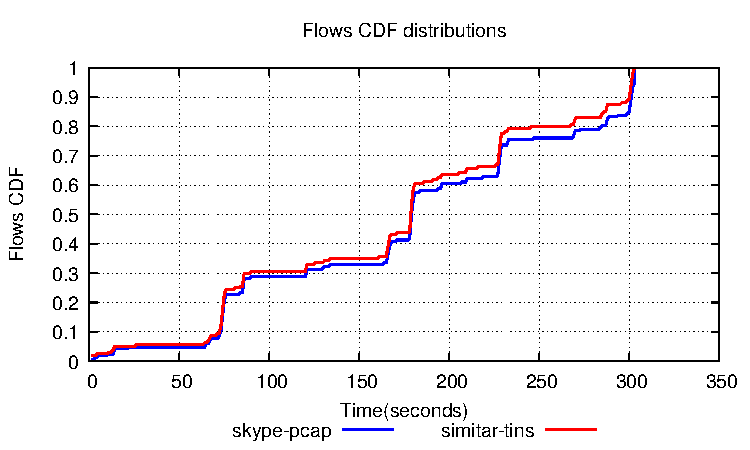
\includegraphics[width=77mm]{figures/ch5/tinsFlowCdf.pdf}
		\label{fig:tins-single-flowcdf}
	}
	\hspace{0mm}
	\subfloat[\textit{wan-pcap}]{
		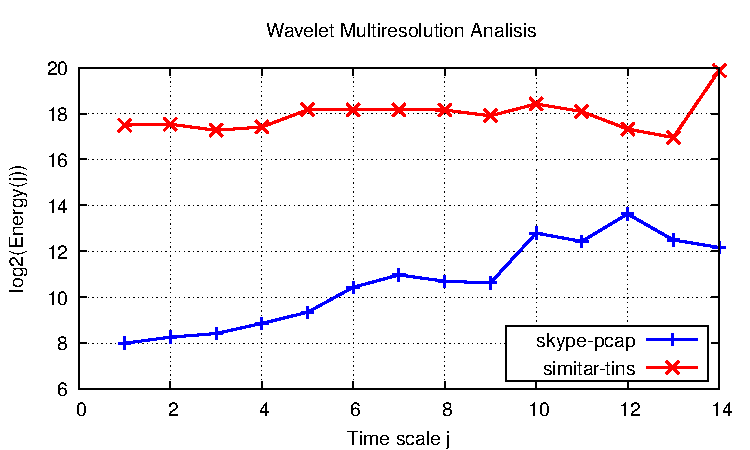
\includegraphics[width=77mm]{figures/ch5/tinsWaveletMREA.pdf}
		\label{fig:tins-single-wavelet}
	}
	\caption{caption}
	\label{fig:tins-single}
\end{figure}



\section{Current Limitations}



To evaluate the Scalling profile of the traccic generator, we are usig the same validation used for Swing\cite{swing-paper}: multiresolution energy analysis.
